\documentclass[12pt]{scrartcl}
\usepackage{setspace}
\usepackage{amsmath}
\usepackage{microtype}
\usepackage{enumitem}
\usepackage{amsmath}
\usepackage{comment}
\usepackage{booktabs}
\usepackage{hyperref}
\usepackage{csquotes}
\usepackage{chemmacros}
\usepackage{graphicx}
\usepackage[utf8]{inputenc}
\usepackage{hyperref}
\MakeOuterQuote{"}
\begin{document}

\title{The Kendall Irrigation Project}
\subtitle{Using Data to Analyze Heterogeneity in Irrigation Patterns and Plant Water Uptake}
\author{Isaac Kramer, Noam Gottlieb, Karin Osadon \\
        The Hebrew University of Jerusalem}
\date{March 2019}
\subject{Needle in a Data Haystack\\
Introduction to Data Science (67978) \\}


%Essay Header
    \pagestyle{myheadings}
    \markright{\hfill \emph{I. Kramer (341352813), N. Gottlieb (201606951), K. Osadon (203057310)}}


\begin{titlepage}
		\maketitle

    \begin{abstract}
    This is the paper's abstract \ldots
    \end{abstract}
\end{titlepage}\setstretch{1.15}


\doublespacing
\section{Introduction}
In recent years, many researchers have identified the potential that data science has to improve resource efficiency and crop yields in agriculture. This is especially true with respect to irrigation management. At present, most irrigation decisions are often made based on the assumption that field conditions are homogenous. Most fields, however, have internal variations in slope, soil depth and type, and aspect, among other variables. This variation can affect the distribution of irrigation water, resulting in certain plants performing better than others.

More accurate knowledge of how heterogeneity affects the distribution of water and plant growth could help both increase plant growth and allow more efficient use of water resources. To this end, a team of researchers at the Volcani Institute is engaged in a multiyear project aimed at increasing our understanding of how spacial heterogeneity within an agriculture field affects the distribution of irrigation water, and how this in turn affects plant production.

During 2017-2018, this team conducted a field experiment in a wine vineyard located within Israel's Judean Hills region (Mevo-Beitar). The area of the vineyard is 2.4 ha and its terrain is highly variable. The vines in the vineyard were planted in 2011 in a northwest-to-southeast direction with a vine and row spacing of 1.5 m and 3.0 m, respectively.

As a part of their ongoing experiment, the researchers divided a section of the vineyard into 10 "zones." Over the course of the growing season, the different zones were subjected to different irrigation regimes and the plant health within each of the zones was measured.

\section{Data}
The research team provided us with the following data associated with this experiment:

\begin{enumerate}
\item Readings from 30 Time-Domain Reflectometry (TDR) sensors. The TDR sensors were used to measure soil volumetric water content, soil temperature, and soil electrical conductivity. Volumetric water content ($\theta$) is defined as $$\theta = \frac{V_w}{V_t}$$ where $V_w$ is the volume of water in a given soil unit and $V_t$ is the total volume of the soil unit (i.e., it includes the volume of air, solid, and water in the soil). Volumetric water content is by definition dimensionless and its values can be reported as a decimal or percent. Electrical conductivity is useful as an indication of the quantity of salts (Na\pch, Ca\pch[2], Mg\pch[2], etc...) in a soil. While many salts are essential to plant development, concentrations above specific thresholds can cause significant declines in plant growth.

The 30 TDR sensors were divided such that three were placed at different locations within each of the 10 zones. Each of the TDR sensors was buried in the soil at a depth of 30 cm. Measurements were recorded every five minutes. We received data corresponding to the three month period beginning in May 2018.

\item Measurements of the Stem Water Potential (SWP) for 30 plants. SWP measurements are useful as an indicator of the degree water stress a plant is experiencing. Readings that are highly negative correspond to high levels of water stress, while readings that are closer to zero indicate that a plant is not experiencing water stress.

Each of the 30 selected plants was adjacent to one of the previously mentioned TDR sensors. The condition of the selected plants should, in theory, reflect the condition of the adjacent soil. The SWP data that we received corresponds to weekly measurements taken during the period from May to July 2018.

\item The quantity of irrigation water supplied to each of zones. Decisions about whether to irrigate each of the given zones were made weekly, based on the SWP measurements. If the SWP measurements indicated the plants in a particular zone were not experiencing water stress, they were not irrigated that week. If the SWP measurements indicated water stress, the plants were irrigated based on the degree of stress exhibited (i.e., more stressed plants larger irrigation inputs than plants with lower levels of stress).

The irrigation quantities were reported in terms of volume of water per dunam (i.e., mm). All irrigation in the vineyard was done using freshwater.

 \item Selected soil properties at the location of the TDR sensors. This data included the aspect, slope, elevation, and total soil depth in the area where each of the TDR sensors was placed.
\end{enumerate}

\section{Objectives}
Our objectives for this project were to mine the dataset to explore possible connections between soil conditions, plant water stress, and soil properties. Specifically, we defined the following sub-objectives:
\begin{itemize}
\item Can we establish a connection between soil water content and the appearance of stress in that plant?
\item Can we determine which soils behave most similarly? For each sensor we have data for the following variables: Water Content, Temperature, and Electrical Conductivity. If we make these three values a vector (i.e., one vector per sensor per time step) can we identify soils that are most similar to each other?
\item Initial analysis of the TDR measurements indicated that following irrigation events, some areas lost water at much faster rates than others. We investigated whether this phenomenon can be connected soil properties (slope and soil depth).
\item more goals, if there are any...
\end{itemize}

\section{Data Cleaning}
Our first step in the project was to do a preliminary clean of the TDR data. We updated the date-time format, simplified the column headers, and ensured cells with missing values were represented uniformly. This was accomplished using the script data\_clean.py.

We continued the data cleaning process by removing values at times when the sensors appeared to be malfunctioning. \autoref{fig:VWC-bad-data} shows plots of the volumetric water content (\%) for each of the 30 sensors during the duration of the measurement period. The plots also show dates of irrigation inputs (mm of water). The script facet\_with\_irrigation.py was used to build these plots. From these plots, we are able to see clearly that certain sensors were not functioning properly. For example, Sensor 1 in Area C shows no response to changes in water content, while Sensor 2 in Area I makes extreme jumps. Before proceeding with our analysis we removed all results from the sensors that did not appear to be working properly.

\begin{figure}[!htb]
        \center{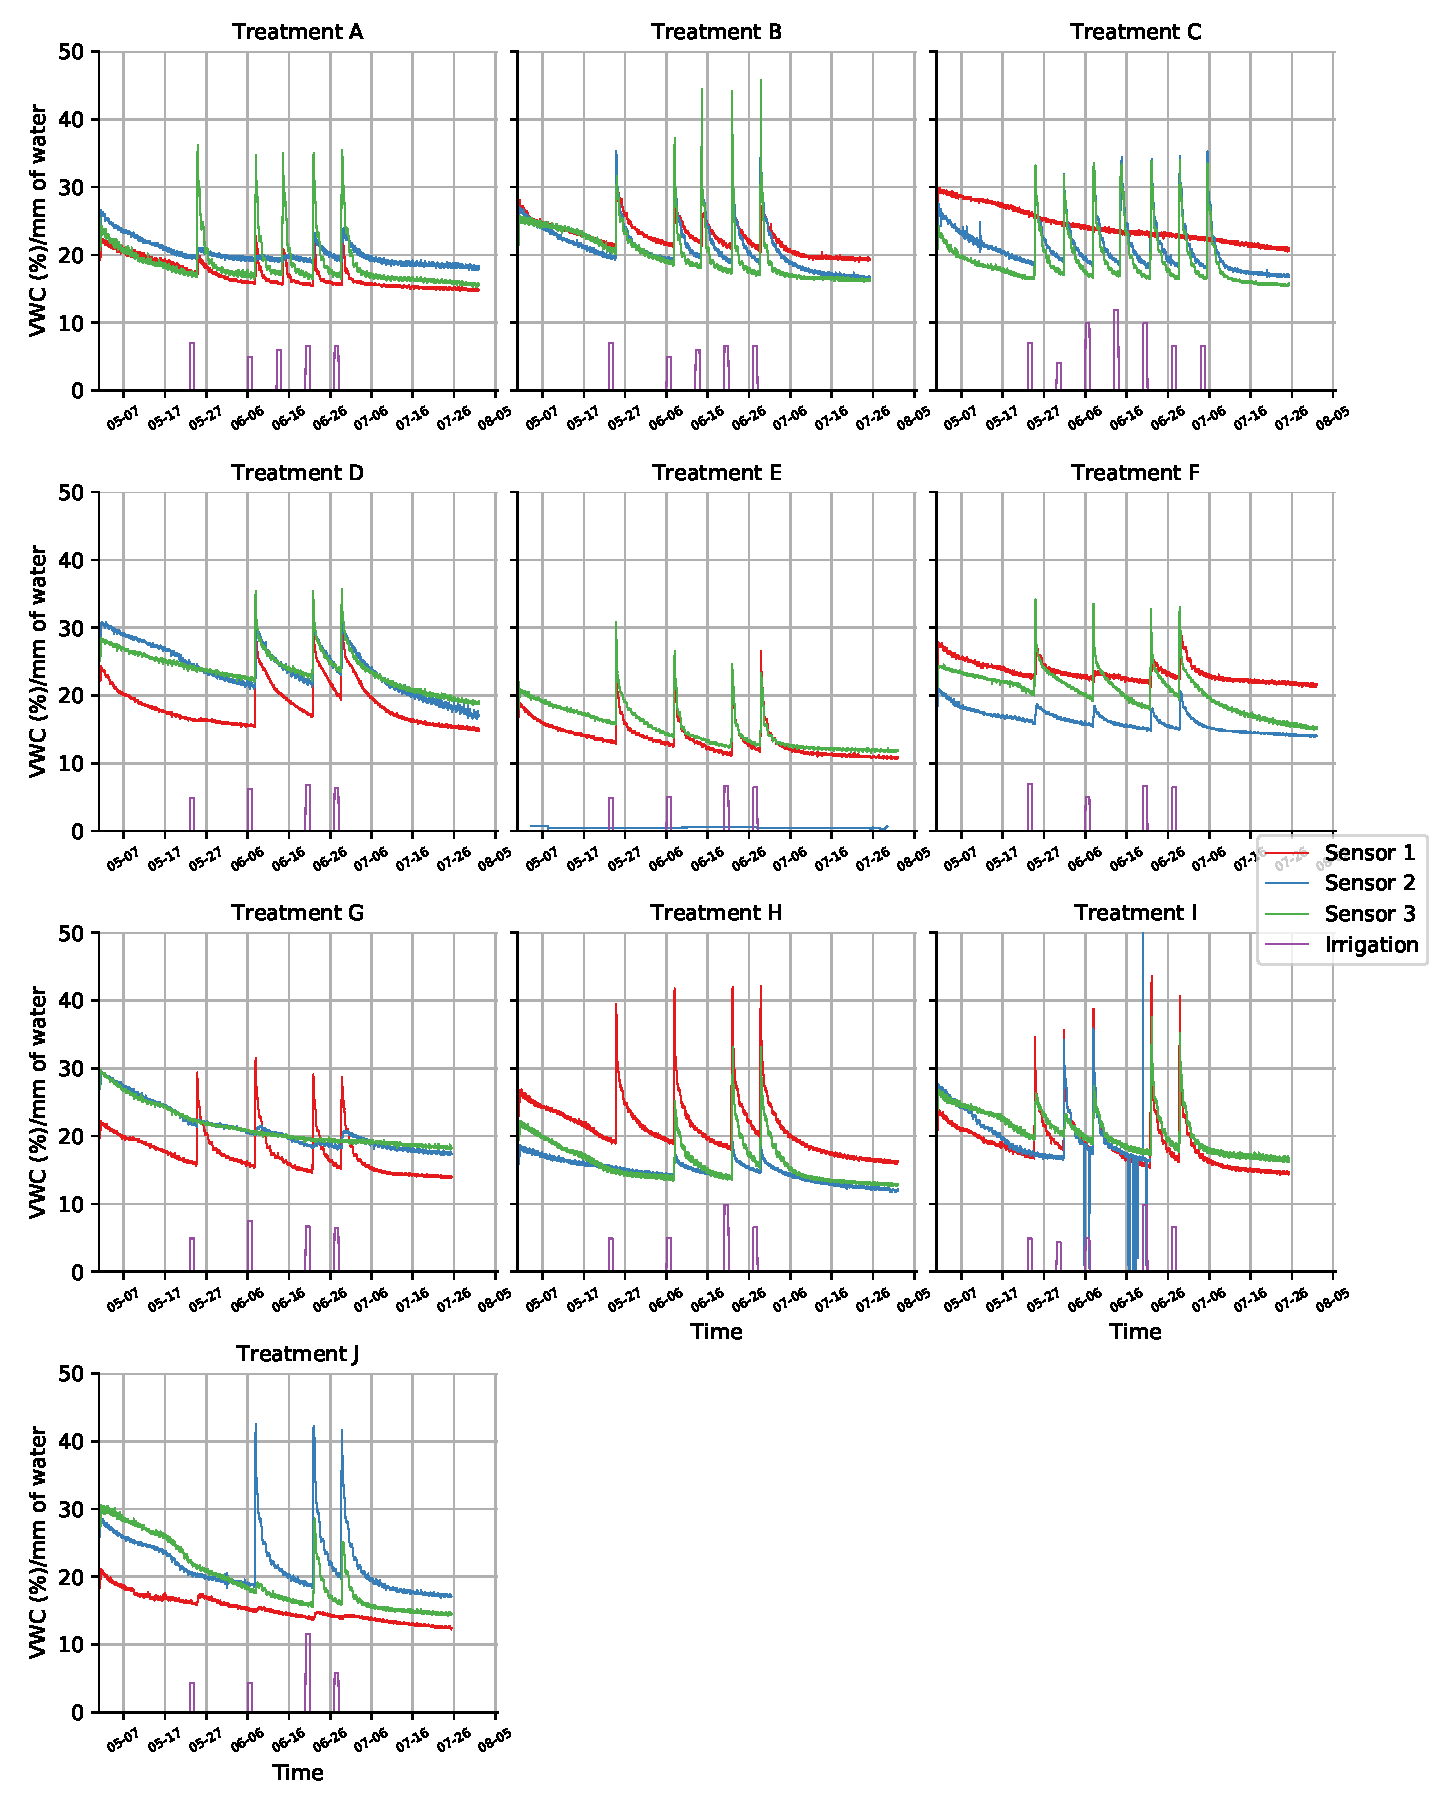
\includegraphics[height=.95\textheight]
        {figures/facet_bad_data.pdf}}
        \caption{\label{fig:VWC-bad-data} Plots showing the volumetric water content and irrigation inputs against time before removing data from malfunctioning sensors. The script facet\_with\_irrigation.py was used to build these plots.}
\end{figure}

\section{Results}
\subsection{Effect of Slope and Soil Depth on Water Loss Rate}
The plots show that some of the soils lose water at a much faster rate following an irrigation event than others. For example, if we compare Areas C and D, we see that the volumetric water content declines much faster for the sensors located in Area C than for the sensors located in Area D. The researchers working on this project hypothesized that one reason for this might be variations in slope and soil depth.

To investigate this question, we wrote a code that calculated the "rate of decline" following an irrigation event (slopes.py). This code identifies the local maxima in water content (i.e., the water content following an irrigation event), as shown in \autoref{fig:irrigation-max}. It then calculates the rate of decline following these events. The code can be adjusted to calculate the rate of decline for a varying amount of time following an irrigation event (e.g., to consider just the first hour after an irrigation event, one day, several days, etc...). Because each sensor experiences multiple irrigation events, the code calculates an average based on each of the events.

\begin{figure}[!htb]
        \center{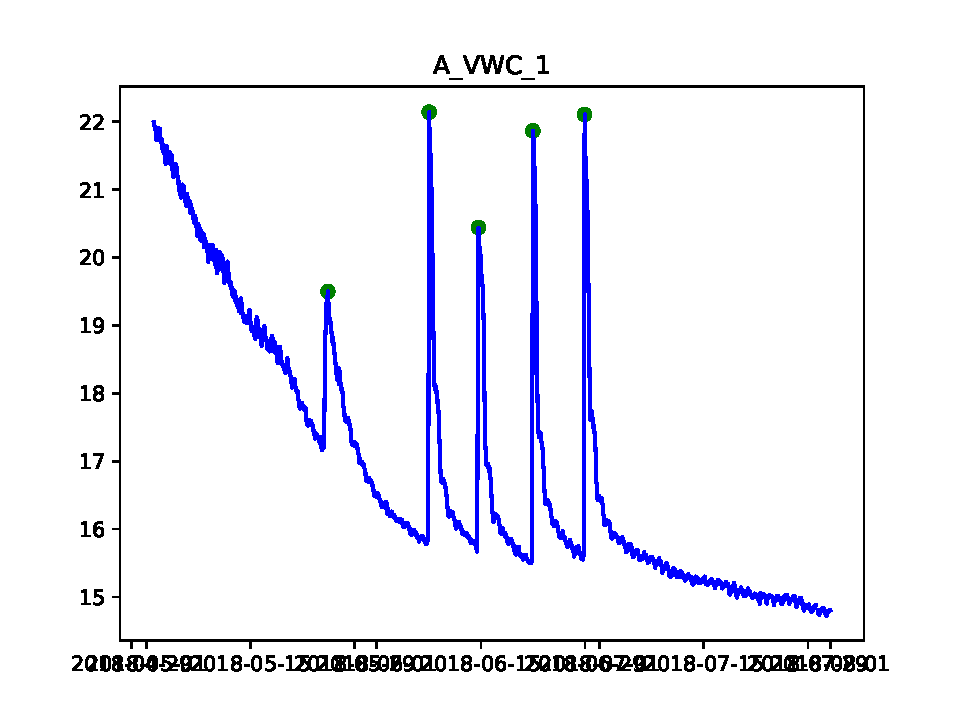
\includegraphics[height=.4\textheight]
        {figures/irrigation_max.pdf}}
        \caption{\label{fig:irrigation-max} Plot showing the maximum volumetric water contents reached for Area A, Sensor 1 as identified by the code in slopes.py}
\end{figure}

Unfortunately, our results showed little connection between the "average loss rate" and the soil slope and/or soil depth. \autoref{fig:slope} includes plots showing the average loss rate following an irrigation event vs. slope and soil depth (cm). As is clear in these plots, no visible relationship exists between the variables. An attempt to build a multiple linear regression model using both slope and soil depth as explanatory variables also produced an R-squared value of nearly 0.0. The results did not change when we varied the length of time following an irrigation maximum used to calculate the average loss rate. 


\begin{figure}[!htb]
    \centering
    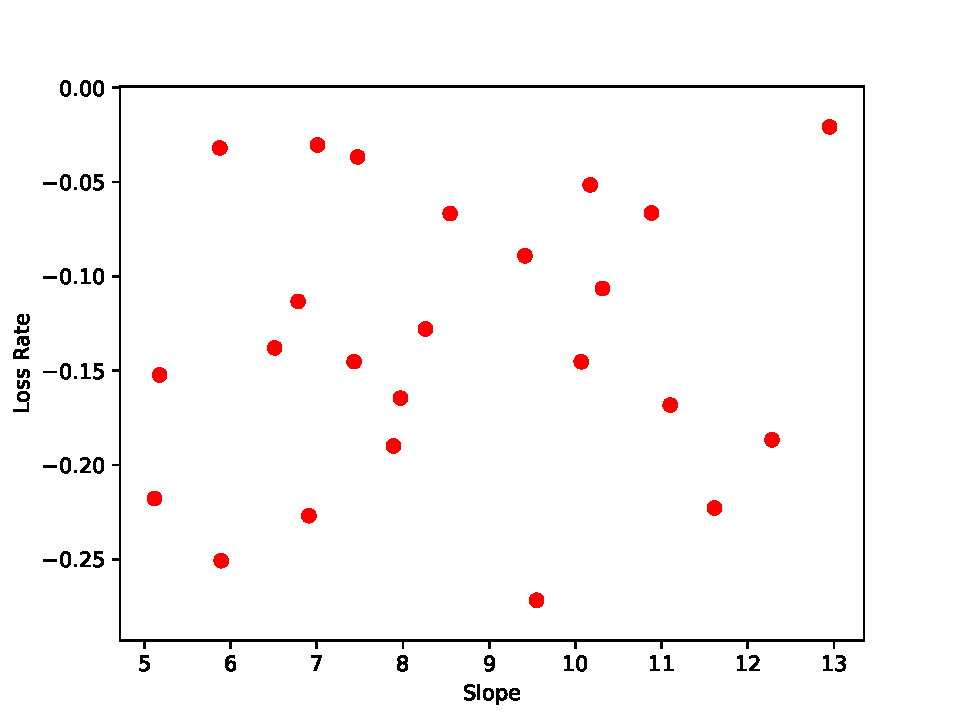
\includegraphics[width=0.495\textwidth]{figures/slope_loss.pdf}
    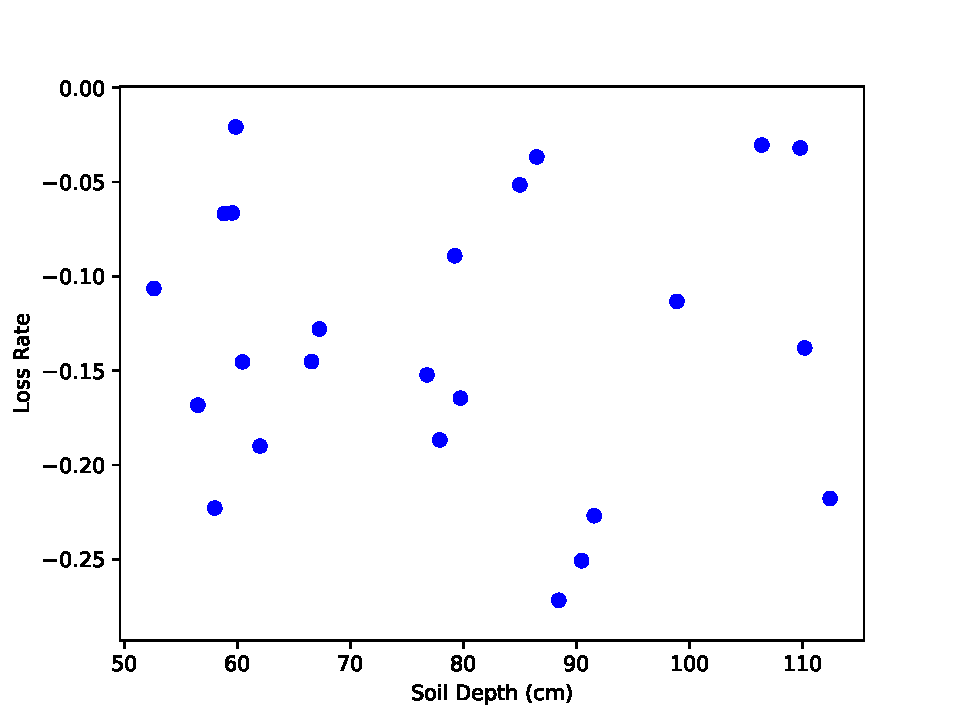
\includegraphics[width=0.495\textwidth]{figures/soil_depth_loss.pdf}
    \caption{Plots showing average loss rate following an irrigation event vs. slope for each of the sensors and soil depth (cm).}
    \label{fig:slope}
\end{figure}






\end{document}
